\documentclass{beamer}
\usetheme{metropolis}
\usepackage{amsmath}
\usepackage{appendixnumberbeamer}
\usepackage{array}
\usepackage{booktabs}
\usepackage{color}
\usepackage{colortbl}
\usepackage{empheq}
\usepackage{ifthen}
\usepackage{keyval}
\usepackage{mathtools}
\usepackage{multirow}
\usepackage{pgfplots}
\usepackage{tabularx}
\usepackage[most]{tcolorbox}
\usepackage{tikz}
\usepackage{upgreek}

\usetikzlibrary{arrows.meta, backgrounds, calc, fit, positioning}

\DeclareMathOperator*{\binop}{\oplus}
\DeclareMathOperator{\sigmoid}{sigmoid}

\newcommand{\binopb}{\ensuremath{\sideset{}{_b}\binop}}
\newcommand{\mutanfeat}[1]{\ensuremath{\tilde{\mathbf{#1}}}}
\renewcommand{\T}{\ensuremath{\mathcal{T}}}
\newcommand{\tuckbranch}{\ensuremath{\T_r^{\q{}\v{}}}}
\newcommand{\q}{\ensuremath{\mathbf{q}}}
\renewcommand{\v}{\ensuremath{\mathbf{v}}}
\newcommand{\qtWq}{\q^\intercal{} W_\q{}}
\newcommand{\vtWv}{\v^\intercal{} W_\v{}}

\newtcbox{\mymath}[1][]{%
    nobeforeafter, math upper, tcbox raise base,
    enhanced, colframe=blue!30!black,
    colback=blue!30, boxrule=1pt,
    #1}

% Presentation flow plan:
%
% Goals:
%
%       0. The idea of presenting my work in this middle stage is to request
%       feedback, ideas and direction from the (extended) group. Focused on how
%       to follow up search space definition with actual search implementation.
%
%
%       To what type of problems can fusion operator search be applied?
%
%       VQA:
%
%       Make the case that this is:
%               1. An important problem.
%               2. A difficult problem (cite tips and tricks paper with
%                  balanced question statistic).
%               3. A problem that current techniques struggle with (see above).
%               4. A problem that automatic fusion operator model selection can
%                  address.
%
%       Give MUTAN as motivation for improving performance by improving the
%       multi-modal fusion operator.
%
%       Expand with my Generalized Hadamard prod paper...
%
%       Other examples of open problems to which fusion operator search can be
%       applied:
%
%       Action recognition in video: the "Revisiting the effectiveness of
%       off-the-shelf temporal modeling approaches for large-scale video
%       classification" Kinetics submission.
%
%       Take advantage of Dhanesh's multi-modal literature review:
%       SIGPROC-Rev1.pdf.
%
%
%       1-?. Present and explain the research on which my proposed research
%       depends?
%
%       1. Related, previous work on same topic from this group:
%
%       ModOut: https://hal.archives-ouvertes.fr/hal-01444614
%
%       Structure Optimization for Deep Multimodal Fusion Networks Using
%       Graph-Induced Kernels: https://arxiv.org/abs/1707.00750.
%
%
%       2a. Architecture search techniques:
%
%       Neural optimizer search with reinforcement learning:
%       http://proceedings.mlr.press/v70/bello17a.html.
%
%       Neural architecture search with reinforcement learning:
%       https://www.openreview.net/pdf?id=r1Ue8Hcxg.
%
%       Learning to learn by gradient descent by gradient descent:
%       https://arxiv.org/abs/1606.04474.
%
%       Meta-learning symposium: http://metalearning-symposium.ml/
%
%
%       2b. Possible ways to apply architecture search to multi-modal fusion
%       problem.
%
%       Ask for ideas, based on what was just presented.
%
%       Ideas:
%               - Use dynamic programming to add layers, finding first the best
%               policy for a single fusion layer, then explore out to >= 2
%               layers.
%                       - Morphisms
%
%               In this case, the current state would be the state of the
%               fusion architecture that has been added on to the original
%               network, and the action space would be where to add the next
%               layer or fusion operation.
%
%               - Action space: join any of N activation map layers from each
%               stream with any other activation map using a fusion operator.
%
%               E.g., combine RGB and optical flow at multiple levels for
%               multiple parallel streams, and fuse those.
%

\title{Automatic Fusion Operator Model Selection for Multimodal Tasks}
\date{\today}
\author{Brendan Duke}
\institute{University of Guelph}

\begin{document}

\maketitle

\begin{frame}{Table of contents}
  \setbeamertemplate{section in toc}[sections numbered]
  \tableofcontents[hideallsubsections]
\end{frame}


% \section{Introduction}

% \begin{frame}[fragile]{Questions to answer}
%         \begin{itemize}[<+- | alert@+>]
%                 \item What is Visual Question-Answering (VQA) and why do we care?
%                         Why is VQA a difficult problem?

%                 \item What are fusion operators, and how can they address the
%                         VQA problem?

%                 \item How might model search techniques be used as methods of
%                         learning fusion operators for VQA\@?
%         \end{itemize}
% \end{frame}


\section{VQA}

{%
% VQA v2 is a hard problem:
% 1. Added ~200K each balancing examples to train and test, 100K to val.
% 2. Balanced examples mined from similar features (in space of VGG-16
%    pre-trained on ImageNet), but have different answer to same question.
\setbeamertemplate{frame footer}{\cite{goyal2017making}}
\begin{frame}{VQA v2}
        \center{}
        % \vspace{-0.8cm}
        \hspace*{-2mm}
        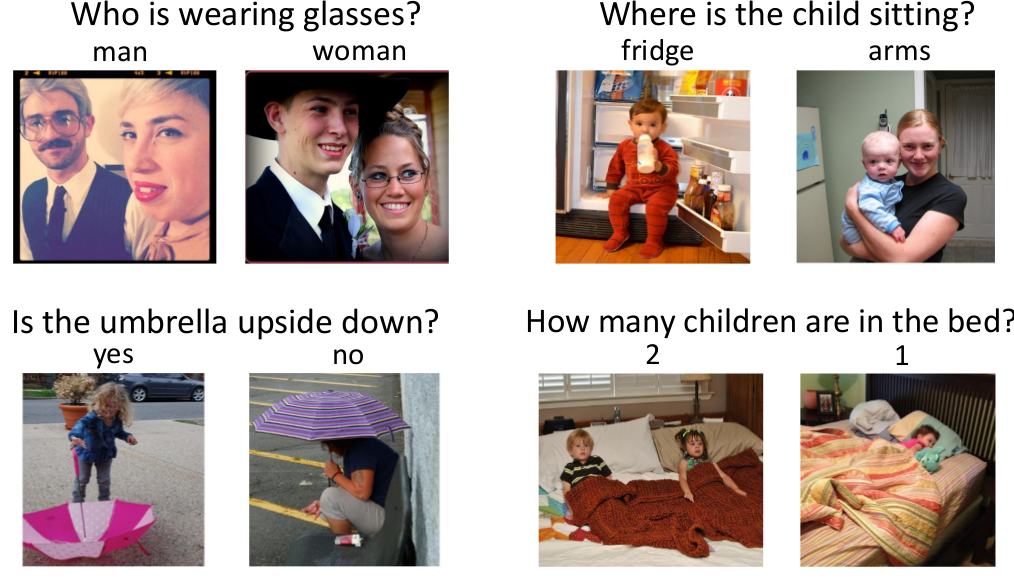
\includegraphics[scale=0.31]{data/vqa2-balanced-imgs}
\end{frame}
}

{%
\setbeamertemplate{frame footer}{\cite{teney2017tips}}
\begin{frame}{VQA v2 balanced pair accuracy}
\center{}
\small
\begin{tabular}{l*{4}{>{$}c<{$}}>{\bfseries}p{8mm}}
        \toprule
        & \multicolumn{4}{c}{VQA v2 validation} & \multirow{3}{8mm}{Acc.\ over pairs}\\
        \cmidrule{2-5}
        & \multicolumn{4}{c}{VQA Score} & \\
        \cmidrule{2-5}
        & All & Yes/no & Num. & Other & \\
        \midrule
        \textbf{Reference Model} & 63.15 \pm{} 0.08 & 80.07 & 42.87 & 55.81 & 34.66 \\
        \midrule
        (1) $w_o^\mathrm{text}$ init. & 63.01 \pm{} 0.12 & 80.11 & 42.80 & 55.51 & 34.40 \\
        (2) $w_o^\mathrm{img}$ init. & 62.67 \pm{} 0.07 & 79.75 & 42.64 & 55.14 & 34.22 \\
        (3) bottom-up attn & 58.90 \pm{} 0.10 & 77.16 & 37.18 & 50.92 & 29.39 \\
        \multicolumn{6}{c}{$\ldots$} \\
        \bottomrule
\end{tabular}
\end{frame}
}


\section{Fusion Operators}

% {%
% % Fibers needed for explanation of mode-i tensor product used in Tucker
% % decomposition, which is the fusion operator in the MUTAN model.
% \setbeamertemplate{frame footer}{\cite{Kolda:2009:TDA:1655228.1655230}}
% \begin{frame}{Tensor mode-$i$ fibers}
%         \center{}
%         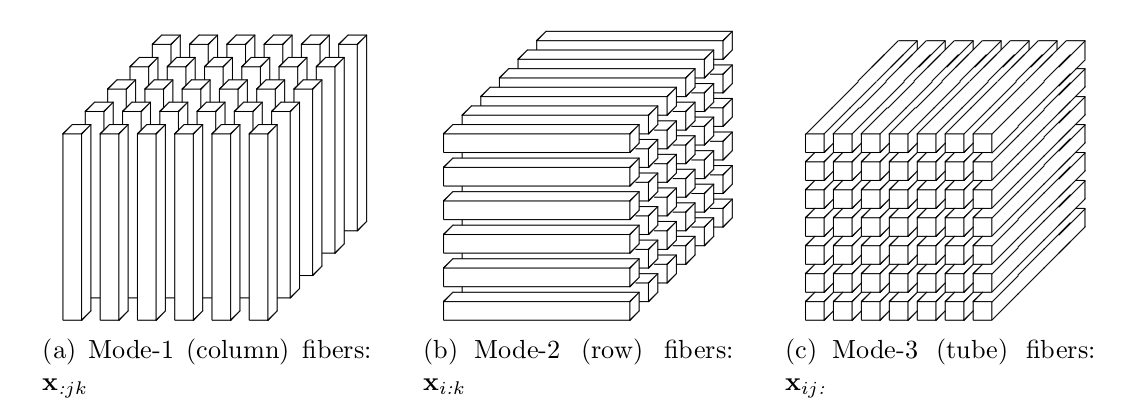
\includegraphics[scale=0.275]{data/tensor_fibers}
% \end{frame}
% }

% {%
% % This is the Tucker decomposition used as the multi-modal fusion operator in
% % MUTAN. Here the matrices A, B and C are analogous to the principal components
% % eigenvectors in PCA.
% \setbeamertemplate{frame footer}{\cite{Kolda:2009:TDA:1655228.1655230}}
% \begin{frame}{Tucker decomposition}
%         \center{}
%         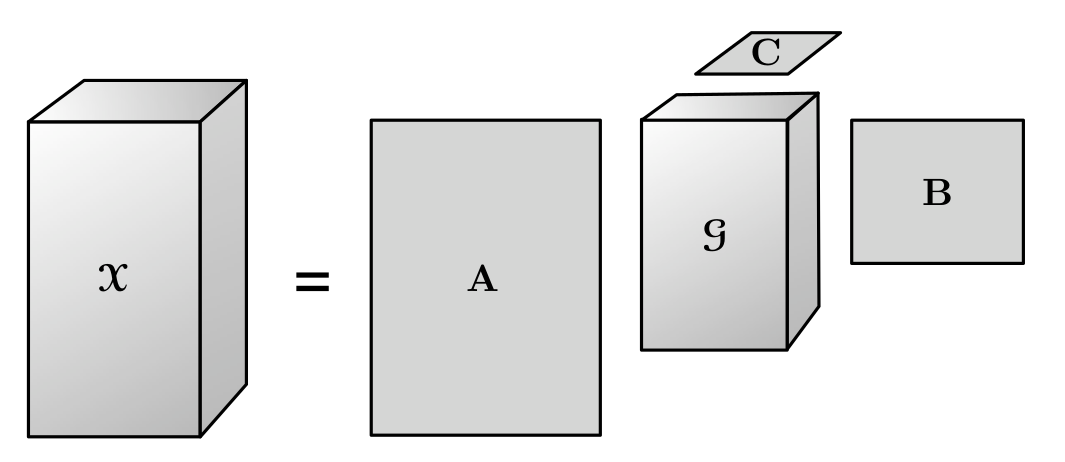
\includegraphics[scale=0.28]{data/tucker_decomp}
%         \begin{equation*}
%                 \mathcal{X} \approx \mathcal{G} \times_1 \mathbf{A} \times_2 \mathbf{B} \times_3 \mathbf{C}
%         \end{equation*}
% \end{frame}
% }

\tcbset{highlight math style={boxsep=5mm,colback=red!30!white}}

{%
% Geometric representation of first two n-mode products
% q^t Wq is combined with Tc via inner product broadcast (matmul)
% ditto for v^t Wv
\begin{frame}{Tensor product}
        \center{}
        % NOTE(brendan): Source:
% https://tex.stackexchange.com/questions/29877/need-help-creating-a-3d-cube-from-a-2d-set-of-nodes-in-tikz

\makeatletter

% Standard Values for Parameters
\newcommand{\tikzcuboid@shiftx}{0}
\newcommand{\tikzcuboid@shifty}{0}
\newcommand{\tikzcuboid@dimx}{3}
\newcommand{\tikzcuboid@dimy}{3}
\newcommand{\tikzcuboid@dimz}{3}
\newcommand{\tikzcuboid@scale}{1}
\newcommand{\tikzcuboid@densityx}{1}
\newcommand{\tikzcuboid@densityy}{1}
\newcommand{\tikzcuboid@densityz}{1}
\newcommand{\tikzcuboid@rotation}{0}
\newcommand{\tikzcuboid@anglex}{0}
\newcommand{\tikzcuboid@angley}{90}
\newcommand{\tikzcuboid@anglez}{225}
\newcommand{\tikzcuboid@scalex}{1}
\newcommand{\tikzcuboid@scaley}{1}
\newcommand{\tikzcuboid@scalez}{sqrt(0.5)}
\newcommand{\tikzcuboid@linefront}{black}
\newcommand{\tikzcuboid@linetop}{black}
\newcommand{\tikzcuboid@lineright}{black}
\newcommand{\tikzcuboid@fillfront}{white}
\newcommand{\tikzcuboid@filltop}{white}
\newcommand{\tikzcuboid@fillright}{white}
\newcommand{\tikzcuboid@shaded}{N}
\newcommand{\tikzcuboid@shadecolor}{black}
\newcommand{\tikzcuboid@shadeperc}{25}
\newcommand{\tikzcuboid@emphedge}{N}
\newcommand{\tikzcuboid@emphstyle}{thick}
\newcommand{\foreachsteppingx}{%
\ifthenelse{\equal{\dimx}{1}}
    {\foreach \x in {\steppingx,...,\dimx}}
    {\foreach \x in {\steppingx,\secondx,...,\dimx}}
}
\newcommand{\foreachsteppingy}{%
\ifthenelse{\equal{\dimy}{1}}
    {\foreach \y in {\steppingy,...,\dimy}}
    {\foreach \y in {\steppingy,\secondy,...,\dimy}}
}
\newcommand{\foreachsteppingz}{%
\ifthenelse{\equal{\dimz}{1}}
    {\foreach \z in {\steppingz,...,\dimz}}
    {\foreach \z in {\steppingz,\secondz,...,\dimz}}
}

% Definition of Keys
\define@key{tikzcuboid}{shiftx}[\tikzcuboid@shiftx]{\renewcommand{\tikzcuboid@shiftx}{#1}}
\define@key{tikzcuboid}{shifty}[\tikzcuboid@shifty]{\renewcommand{\tikzcuboid@shifty}{#1}}
\define@key{tikzcuboid}{dimx}[\tikzcuboid@dimx]{\renewcommand{\tikzcuboid@dimx}{#1}}
\define@key{tikzcuboid}{dimy}[\tikzcuboid@dimy]{\renewcommand{\tikzcuboid@dimy}{#1}}
\define@key{tikzcuboid}{dimz}[\tikzcuboid@dimz]{\renewcommand{\tikzcuboid@dimz}{#1}}
\define@key{tikzcuboid}{scale}[\tikzcuboid@scale]{\renewcommand{\tikzcuboid@scale}{#1}}
\define@key{tikzcuboid}{densityx}[\tikzcuboid@densityx]{\renewcommand{\tikzcuboid@densityx}{#1}}
\define@key{tikzcuboid}{densityy}[\tikzcuboid@densityy]{\renewcommand{\tikzcuboid@densityy}{#1}}
\define@key{tikzcuboid}{densityz}[\tikzcuboid@densityz]{\renewcommand{\tikzcuboid@densityz}{#1}}
\define@key{tikzcuboid}{rotation}[\tikzcuboid@rotation]{\renewcommand{\tikzcuboid@rotation}{#1}}
\define@key{tikzcuboid}{anglex}[\tikzcuboid@anglex]{\renewcommand{\tikzcuboid@anglex}{#1}}
\define@key{tikzcuboid}{angley}[\tikzcuboid@angley]{\renewcommand{\tikzcuboid@angley}{#1}}
\define@key{tikzcuboid}{anglez}[\tikzcuboid@anglez]{\renewcommand{\tikzcuboid@anglez}{#1}}
\define@key{tikzcuboid}{scalex}[\tikzcuboid@scalex]{\renewcommand{\tikzcuboid@scalex}{#1}}
\define@key{tikzcuboid}{scaley}[\tikzcuboid@scaley]{\renewcommand{\tikzcuboid@scaley}{#1}}
\define@key{tikzcuboid}{scalez}[\tikzcuboid@scalez]{\renewcommand{\tikzcuboid@scalez}{#1}}
\define@key{tikzcuboid}{linefront}[\tikzcuboid@linefront]{\renewcommand{\tikzcuboid@linefront}{#1}}
\define@key{tikzcuboid}{linetop}[\tikzcuboid@linetop]{\renewcommand{\tikzcuboid@linetop}{#1}}
\define@key{tikzcuboid}{lineright}[\tikzcuboid@lineright]{\renewcommand{\tikzcuboid@lineright}{#1}}
\define@key{tikzcuboid}{fillfront}[\tikzcuboid@fillfront]{\renewcommand{\tikzcuboid@fillfront}{#1}}
\define@key{tikzcuboid}{filltop}[\tikzcuboid@filltop]{\renewcommand{\tikzcuboid@filltop}{#1}}
\define@key{tikzcuboid}{fillright}[\tikzcuboid@fillright]{\renewcommand{\tikzcuboid@fillright}{#1}}
\define@key{tikzcuboid}{shaded}[\tikzcuboid@shaded]{\renewcommand{\tikzcuboid@shaded}{#1}}
\define@key{tikzcuboid}{shadecolor}[\tikzcuboid@shadecolor]{\renewcommand{\tikzcuboid@shadecolor}{#1}}
\define@key{tikzcuboid}{shadeperc}[\tikzcuboid@shadeperc]{\renewcommand{\tikzcuboid@shadeperc}{#1}}
\define@key{tikzcuboid}{emphedge}[\tikzcuboid@emphedge]{\renewcommand{\tikzcuboid@emphedge}{#1}}
\define@key{tikzcuboid}{emphstyle}[\tikzcuboid@emphstyle]{\renewcommand{\tikzcuboid@emphstyle}{#1}}
% Commands
\newcommand{\tikzcuboid}[1]{
    \setkeys{tikzcuboid}{#1} % Process Keys passed to command
    \pgfmathsetmacro{\vectorxx}{\tikzcuboid@scalex*cos(\tikzcuboid@anglex)}
    \pgfmathsetmacro{\vectorxy}{\tikzcuboid@scalex*sin(\tikzcuboid@anglex)}
    \pgfmathsetmacro{\vectoryx}{\tikzcuboid@scaley*cos(\tikzcuboid@angley)}
    \pgfmathsetmacro{\vectoryy}{\tikzcuboid@scaley*sin(\tikzcuboid@angley)}
    \pgfmathsetmacro{\vectorzx}{\tikzcuboid@scalez*cos(\tikzcuboid@anglez)}
    \pgfmathsetmacro{\vectorzy}{\tikzcuboid@scalez*sin(\tikzcuboid@anglez)}
    \begin{scope}[xshift=\tikzcuboid@shiftx, yshift=\tikzcuboid@shifty, scale=\tikzcuboid@scale, rotate=\tikzcuboid@rotation, x={(\vectorxx,\vectorxy)}, y={(\vectoryx,\vectoryy)}, z={(\vectorzx,\vectorzy)}]
    \pgfmathsetmacro{\steppingx}{1/\tikzcuboid@densityx}
    \pgfmathsetmacro{\steppingy}{1/\tikzcuboid@densityy}
    \pgfmathsetmacro{\steppingz}{1/\tikzcuboid@densityz}
    \newcommand{\dimx}{\tikzcuboid@dimx}
    \newcommand{\dimy}{\tikzcuboid@dimy}
    \newcommand{\dimz}{\tikzcuboid@dimz}
    \pgfmathsetmacro{\secondx}{2*\steppingx}
    \pgfmathsetmacro{\secondy}{2*\steppingy}
    \pgfmathsetmacro{\secondz}{2*\steppingz}
    \foreachsteppingx
    {
        \foreachsteppingy
        {   \pgfmathsetmacro{\lowx}{(\x-\steppingx)}
            \pgfmathsetmacro{\lowy}{(\y-\steppingy)}
            \filldraw[fill=\tikzcuboid@fillfront,draw=\tikzcuboid@linefront] (\lowx,\lowy,\dimz) -- (\lowx,\y,\dimz) -- (\x,\y,\dimz) -- (\x,\lowy,\dimz) -- cycle;

        }
    }
    \foreachsteppingx
    {
        \foreachsteppingz
        {   \pgfmathsetmacro{\lowx}{(\x-\steppingx)}
            \pgfmathsetmacro{\lowz}{(\z-\steppingz)}
            \filldraw[fill=\tikzcuboid@filltop,draw=\tikzcuboid@linetop] (\lowx,\dimy,\lowz) -- (\lowx,\dimy,\z) -- (\x,\dimy,\z) -- (\x,\dimy,\lowz) -- cycle;
        }
    }
    \foreachsteppingy
    {
        \foreachsteppingz
        {   \pgfmathsetmacro{\lowy}{(\y-\steppingy)}
            \pgfmathsetmacro{\lowz}{(\z-\steppingz)}
            \filldraw[fill=\tikzcuboid@fillright,draw=\tikzcuboid@lineright] (\dimx,\lowy,\lowz) -- (\dimx,\lowy,\z) -- (\dimx,\y,\z) -- (\dimx,\y,\lowz) -- cycle;
        }
    }
    \ifthenelse{\equal{\tikzcuboid@emphedge}{Y}}%
        {\draw[\tikzcuboid@emphstyle](0,\dimy,0) -- (\dimx,\dimy,0) -- (\dimx,\dimy,\dimz) -- (0,\dimy,\dimz) -- cycle;%
        \draw[\tikzcuboid@emphstyle] (0,0,\dimz) -- (0,\dimy,\dimz) -- (\dimx,\dimy,\dimz) -- (\dimx,0,\dimz) -- cycle;%
        \draw[\tikzcuboid@emphstyle](\dimx,0,0) -- (\dimx,\dimy,0) -- (\dimx,\dimy,\dimz) -- (\dimx,0,\dimz) -- cycle;%
        }%
        {}
    \end{scope}
}

\newcommand{\qvectikzdim}{5}
\newcommand{\vvectikzdim}{4}
\newcommand{\cuboidscale}{0.35}


\begin{tikzpicture}
        % NOTE(brendan): Tc
        \tikzcuboid{%
            shiftx=0cm,%
            shifty=0cm,%
            scale=\cuboidscale,%
            rotation=0,%
            densityx=1,%
            densityy=1,%
            densityz=1,%
            dimx=\qvectikzdim,%
            dimy=\vvectikzdim,%
            dimz=3,%
            linefront=black,%
            linetop=black,%
            lineright=black,%
            fillfront=red!50,%
            filltop=green!50,%
            fillright=blue!50,%
            anglex=180,%
            angley=90,%
            anglez=225,%
            scalex=1,%
            scaley=0.8,%
            scalez=0.6,%
            emphedge=N,%
        }

        % NOTE(brendan):
        \tikzcuboid{%
            shiftx=2.0cm,%
            shifty=0cm,%
            scale=\cuboidscale,%
            rotation=0,%
            densityx=1,%
            densityy=1,%
            densityz=1,%
            dimx=1,%
            dimy=\vvectikzdim,%
            dimz=3,%
            linefront=black,%
            linetop=black,%
            lineright=black,%
            fillfront=red!50,%
            filltop=green!50,%
            fillright=blue!50,%
            anglex=180,%
            angley=90,%
            anglez=225,%
            scalex=1,%
            scaley=0.8,%
            scalez=0.6,%
            emphedge=N,%
        }

        \tikzcuboid{%
            shiftx=10pt,%
            shifty=-15mm,%
            scale=\cuboidscale,%
            rotation=0,%
            densityx=1,%
            densityy=1,%
            densityz=1,%
            dimx=\qvectikzdim,%
            dimy=1,%
            dimz=1,%
            linefront=black,%
            linetop=black,%
            lineright=black,%
            fillfront=red!50,%
            filltop=red!50,%
            fillright=red!50,%
            anglex=180,%
            angley=90,%
            anglez=225,%
            scalex=1,%
            scaley=0.8,%
            scalez=0.6,%
            emphedge=N,%
        }

        \newcommand{\qbracesize}{8.5ex}
        \newcommand{\vbracesize}{5ex}

        \coordinate (qbrace) at (-0.35, -1.77);
        \node at (qbrace) {\makebox[\qbracesize]{\upbracefill}};
        \node at (qbrace) [below] {$t_q$};

        \coordinate (Tcq brace) at (-0.42, -0.18);
        \node at (Tcq brace) {\rotatebox{180}{\makebox[\qbracesize]{\upbracefill}}};
        \node[inner sep=1pt] at (Tcq brace) [above, fill=white, fill opacity=0.8, text opacity=1, yshift=1.1mm] {$t_q$};

        \node (Tc label) at (Tcq brace) [xshift=-3mm, yshift=18mm] {$\T_c$};
        \node (Tcq label) at (Tc label) [xshift=27mm] {$\T_c^\q$};
        \node (vtWv label) at (Tc label) [xshift=45mm] {$\vtWv$};
        \node[inner sep=0pt] (qtWq label) at (Tc label) [yshift=-43mm, xshift=3mm] {$\qtWq$};
        \node (Tcqv label) at (Tc label) [xshift=65mm] {$\T_c^{\q\v}$};

        \newcommand{\Tcvy}{0.56}
        \coordinate (Tcv brace) at (-1.9, \Tcvy);
        \node at (Tcv brace) {\rotatebox{270}{\makebox[\vbracesize]{\upbracefill}}};
        \node at (Tcv brace) [left] {$t_v$};

        \coordinate (Tco brace) at (0.33, 1.05);
        \node at (Tco brace) {\rotatebox{140}{\makebox[2ex]{\upbracefill}}};
        \node at (Tco brace) [right, yshift=2.0mm, xshift=-1.0mm] {$t_o$};

        \node at (qbrace) [yshift=10mm] {$\times_1$};

        \tikzcuboid{%
            shiftx=3.8cm,%
            shifty=-7pt,%
            scale=\cuboidscale,%
            rotation=0,%
            densityx=1,%
            densityy=1,%
            densityz=1,%
            dimx=1,%
            dimy=\vvectikzdim,%
            dimz=1,%
            linefront=black,%
            linetop=black,%
            lineright=black,%
            fillfront=blue!50,%
            filltop=blue!50,%
            fillright=blue!50,%
            anglex=180,%
            angley=90,%
            anglez=225,%
            scalex=1,%
            scaley=0.8,%
            scalez=0.6,%
            emphedge=N,%
        }

        \coordinate (vbrace) at (4.1, 0.18);
        \node at (vbrace) {\rotatebox{90}{\makebox[\vbracesize]{\upbracefill}}};
        \node at (vbrace) [right] {$t_v$};

        \draw[->, thick, >= stealth] (0.85, 0.25) -- (1.35, 0.25) {};

        \node at (vbrace) [xshift=-11.5mm, yshift=0mm] {$\times_2$};

        \coordinate (tcqv pos) at (5.7, 0.31);

        \draw[->, thick, >= stealth] (4.63, 0.25) -- (5.13, 0.25) {};

        \tikzcuboid{%
            shiftx=5.76cm,%
            shifty=0.3cm,%
            scale=\cuboidscale,%
            rotation=0,%
            densityx=1,%
            densityy=1,%
            densityz=1,%
            dimx=1,%
            dimy=1,%
            dimz=3,%
            linefront=black,%
            linetop=black,%
            lineright=black,%
            fillfront=red!50,%
            filltop=green!50,%
            fillright=blue!50,%
            anglex=180,%
            angley=90,%
            anglez=225,%
            scalex=1,%
            scaley=0.8,%
            scalez=0.6,%
            emphedge=N,%
        }
\end{tikzpicture}


\begin{empheq}[box=\tcbhighmath]{equation*}
        \T \approx \T_c \times_1 \qtWq \times_2 \vtWv \times_3 W_o
\end{empheq}
\end{frame}
}

{%
% The full MUTAN pipeline for VQA, which we build upon
% (Tc is the rectangle)
\setbeamertemplate{frame footer}{\cite{ben2017mutan}}
\begin{frame}{MUTAN}
        \center{}
        \hspace*{-1.0cm}
        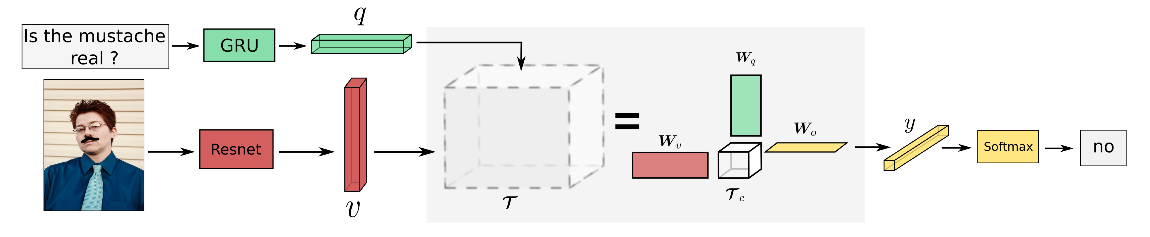
\includegraphics[scale=0.31]{data/mutan}
\end{frame}
}

%{%
%% Contrast of the Tucker decomposition with Multimodal Compact Bilinear (MCB)
%% and Multimodal Low-rank Bilinear (MLB).
%%
%% On the val split of the VQA dataset, the full MUTAN method achieved
%% performance of 58.16 overall as compared with the next best result, 57.94
%% from MLB, and compared with 56.92 from a baseline that just concatenates v
%% and q.
%\setbeamertemplate{frame footer}{\cite{ben2017mutan}}
%\begin{frame}{MCB vs. MLB vs. MUTAN}
%        \center{}
%        \hspace*{-0.9cm}
%        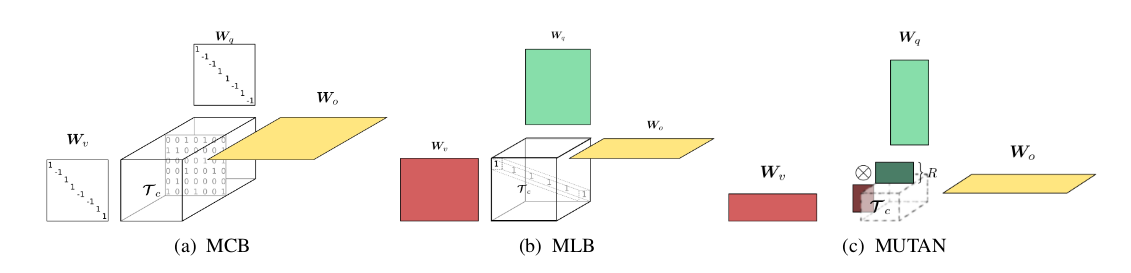
\includegraphics[scale=0.31]{data/mcb_mlb_mutan}
%\end{frame}
%}

{%
% Our generalized fusion operator:
% 1. Nonlinearity ensembling
% 2. Mini-network
% 3. Tree fusion with arbitrary binary ops
\begin{frame}{Generalized fusion operator}
\center{}
\hspace*{-6.0cm}
\scalebox{0.75}{%
% NOTE(brendan): Source:
% https://tex.stackexchange.com/questions/29877/need-help-creating-a-3d-cube-from-a-2d-set-of-nodes-in-tikz

\makeatletter

% Standard Values for Parameters
\newcommand{\tikzcuboid@shiftx}{0}
\newcommand{\tikzcuboid@shifty}{0}
\newcommand{\tikzcuboid@dimx}{3}
\newcommand{\tikzcuboid@dimy}{3}
\newcommand{\tikzcuboid@dimz}{3}
\newcommand{\tikzcuboid@scale}{1}
\newcommand{\tikzcuboid@densityx}{1}
\newcommand{\tikzcuboid@densityy}{1}
\newcommand{\tikzcuboid@densityz}{1}
\newcommand{\tikzcuboid@rotation}{0}
\newcommand{\tikzcuboid@anglex}{0}
\newcommand{\tikzcuboid@angley}{90}
\newcommand{\tikzcuboid@anglez}{225}
\newcommand{\tikzcuboid@scalex}{1}
\newcommand{\tikzcuboid@scaley}{1}
\newcommand{\tikzcuboid@scalez}{sqrt(0.5)}
\newcommand{\tikzcuboid@linefront}{black}
\newcommand{\tikzcuboid@linetop}{black}
\newcommand{\tikzcuboid@lineright}{black}
\newcommand{\tikzcuboid@fillfront}{white}
\newcommand{\tikzcuboid@filltop}{white}
\newcommand{\tikzcuboid@fillright}{white}
\newcommand{\tikzcuboid@shaded}{N}
\newcommand{\tikzcuboid@shadecolor}{black}
\newcommand{\tikzcuboid@shadeperc}{25}
\newcommand{\tikzcuboid@emphedge}{N}
\newcommand{\tikzcuboid@emphstyle}{thick}
\newcommand{\foreachsteppingx}{%
\ifthenelse{\equal{\dimx}{1}}
    {\foreach \x in {\steppingx,...,\dimx}}
    {\foreach \x in {\steppingx,\secondx,...,\dimx}}
}
\newcommand{\foreachsteppingy}{%
\ifthenelse{\equal{\dimy}{1}}
    {\foreach \y in {\steppingy,...,\dimy}}
    {\foreach \y in {\steppingy,\secondy,...,\dimy}}
}
\newcommand{\foreachsteppingz}{%
\ifthenelse{\equal{\dimz}{1}}
    {\foreach \z in {\steppingz,...,\dimz}}
    {\foreach \z in {\steppingz,\secondz,...,\dimz}}
}

% Definition of Keys
\define@key{tikzcuboid}{shiftx}[\tikzcuboid@shiftx]{\renewcommand{\tikzcuboid@shiftx}{#1}}
\define@key{tikzcuboid}{shifty}[\tikzcuboid@shifty]{\renewcommand{\tikzcuboid@shifty}{#1}}
\define@key{tikzcuboid}{dimx}[\tikzcuboid@dimx]{\renewcommand{\tikzcuboid@dimx}{#1}}
\define@key{tikzcuboid}{dimy}[\tikzcuboid@dimy]{\renewcommand{\tikzcuboid@dimy}{#1}}
\define@key{tikzcuboid}{dimz}[\tikzcuboid@dimz]{\renewcommand{\tikzcuboid@dimz}{#1}}
\define@key{tikzcuboid}{scale}[\tikzcuboid@scale]{\renewcommand{\tikzcuboid@scale}{#1}}
\define@key{tikzcuboid}{densityx}[\tikzcuboid@densityx]{\renewcommand{\tikzcuboid@densityx}{#1}}
\define@key{tikzcuboid}{densityy}[\tikzcuboid@densityy]{\renewcommand{\tikzcuboid@densityy}{#1}}
\define@key{tikzcuboid}{densityz}[\tikzcuboid@densityz]{\renewcommand{\tikzcuboid@densityz}{#1}}
\define@key{tikzcuboid}{rotation}[\tikzcuboid@rotation]{\renewcommand{\tikzcuboid@rotation}{#1}}
\define@key{tikzcuboid}{anglex}[\tikzcuboid@anglex]{\renewcommand{\tikzcuboid@anglex}{#1}}
\define@key{tikzcuboid}{angley}[\tikzcuboid@angley]{\renewcommand{\tikzcuboid@angley}{#1}}
\define@key{tikzcuboid}{anglez}[\tikzcuboid@anglez]{\renewcommand{\tikzcuboid@anglez}{#1}}
\define@key{tikzcuboid}{scalex}[\tikzcuboid@scalex]{\renewcommand{\tikzcuboid@scalex}{#1}}
\define@key{tikzcuboid}{scaley}[\tikzcuboid@scaley]{\renewcommand{\tikzcuboid@scaley}{#1}}
\define@key{tikzcuboid}{scalez}[\tikzcuboid@scalez]{\renewcommand{\tikzcuboid@scalez}{#1}}
\define@key{tikzcuboid}{linefront}[\tikzcuboid@linefront]{\renewcommand{\tikzcuboid@linefront}{#1}}
\define@key{tikzcuboid}{linetop}[\tikzcuboid@linetop]{\renewcommand{\tikzcuboid@linetop}{#1}}
\define@key{tikzcuboid}{lineright}[\tikzcuboid@lineright]{\renewcommand{\tikzcuboid@lineright}{#1}}
\define@key{tikzcuboid}{fillfront}[\tikzcuboid@fillfront]{\renewcommand{\tikzcuboid@fillfront}{#1}}
\define@key{tikzcuboid}{filltop}[\tikzcuboid@filltop]{\renewcommand{\tikzcuboid@filltop}{#1}}
\define@key{tikzcuboid}{fillright}[\tikzcuboid@fillright]{\renewcommand{\tikzcuboid@fillright}{#1}}
\define@key{tikzcuboid}{shaded}[\tikzcuboid@shaded]{\renewcommand{\tikzcuboid@shaded}{#1}}
\define@key{tikzcuboid}{shadecolor}[\tikzcuboid@shadecolor]{\renewcommand{\tikzcuboid@shadecolor}{#1}}
\define@key{tikzcuboid}{shadeperc}[\tikzcuboid@shadeperc]{\renewcommand{\tikzcuboid@shadeperc}{#1}}
\define@key{tikzcuboid}{emphedge}[\tikzcuboid@emphedge]{\renewcommand{\tikzcuboid@emphedge}{#1}}
\define@key{tikzcuboid}{emphstyle}[\tikzcuboid@emphstyle]{\renewcommand{\tikzcuboid@emphstyle}{#1}}
% Commands
\newcommand{\tikzcuboid}[1]{
    \setkeys{tikzcuboid}{#1} % Process Keys passed to command
    \pgfmathsetmacro{\vectorxx}{\tikzcuboid@scalex*cos(\tikzcuboid@anglex)}
    \pgfmathsetmacro{\vectorxy}{\tikzcuboid@scalex*sin(\tikzcuboid@anglex)}
    \pgfmathsetmacro{\vectoryx}{\tikzcuboid@scaley*cos(\tikzcuboid@angley)}
    \pgfmathsetmacro{\vectoryy}{\tikzcuboid@scaley*sin(\tikzcuboid@angley)}
    \pgfmathsetmacro{\vectorzx}{\tikzcuboid@scalez*cos(\tikzcuboid@anglez)}
    \pgfmathsetmacro{\vectorzy}{\tikzcuboid@scalez*sin(\tikzcuboid@anglez)}
    \begin{scope}[xshift=\tikzcuboid@shiftx, yshift=\tikzcuboid@shifty, scale=\tikzcuboid@scale, rotate=\tikzcuboid@rotation, x={(\vectorxx,\vectorxy)}, y={(\vectoryx,\vectoryy)}, z={(\vectorzx,\vectorzy)}]
    \pgfmathsetmacro{\steppingx}{1/\tikzcuboid@densityx}
    \pgfmathsetmacro{\steppingy}{1/\tikzcuboid@densityy}
    \pgfmathsetmacro{\steppingz}{1/\tikzcuboid@densityz}
    \newcommand{\dimx}{\tikzcuboid@dimx}
    \newcommand{\dimy}{\tikzcuboid@dimy}
    \newcommand{\dimz}{\tikzcuboid@dimz}
    \pgfmathsetmacro{\secondx}{2*\steppingx}
    \pgfmathsetmacro{\secondy}{2*\steppingy}
    \pgfmathsetmacro{\secondz}{2*\steppingz}
    \foreachsteppingx
    {
        \foreachsteppingy
        {   \pgfmathsetmacro{\lowx}{(\x-\steppingx)}
            \pgfmathsetmacro{\lowy}{(\y-\steppingy)}
            \filldraw[fill=\tikzcuboid@fillfront,draw=\tikzcuboid@linefront] (\lowx,\lowy,\dimz) -- (\lowx,\y,\dimz) -- (\x,\y,\dimz) -- (\x,\lowy,\dimz) -- cycle;

        }
    }
    \foreachsteppingx
    {
        \foreachsteppingz
        {   \pgfmathsetmacro{\lowx}{(\x-\steppingx)}
            \pgfmathsetmacro{\lowz}{(\z-\steppingz)}
            \filldraw[fill=\tikzcuboid@filltop,draw=\tikzcuboid@linetop] (\lowx,\dimy,\lowz) -- (\lowx,\dimy,\z) -- (\x,\dimy,\z) -- (\x,\dimy,\lowz) -- cycle;
        }
    }
    \foreachsteppingy
    {
        \foreachsteppingz
        {   \pgfmathsetmacro{\lowy}{(\y-\steppingy)}
            \pgfmathsetmacro{\lowz}{(\z-\steppingz)}
            \filldraw[fill=\tikzcuboid@fillright,draw=\tikzcuboid@lineright] (\dimx,\lowy,\lowz) -- (\dimx,\lowy,\z) -- (\dimx,\y,\z) -- (\dimx,\y,\lowz) -- cycle;
        }
    }
    \ifthenelse{\equal{\tikzcuboid@emphedge}{Y}}%
        {\draw[\tikzcuboid@emphstyle](0,\dimy,0) -- (\dimx,\dimy,0) -- (\dimx,\dimy,\dimz) -- (0,\dimy,\dimz) -- cycle;%
        \draw[\tikzcuboid@emphstyle] (0,0,\dimz) -- (0,\dimy,\dimz) -- (\dimx,\dimy,\dimz) -- (\dimx,0,\dimz) -- cycle;%
        \draw[\tikzcuboid@emphstyle](\dimx,0,0) -- (\dimx,\dimy,0) -- (\dimx,\dimy,\dimz) -- (\dimx,0,\dimz) -- cycle;%
        }%
        {}
    \end{scope}
}

\newcommand{\qvectikzdim}{5}
\newcommand{\vvectikzdim}{4}
\newcommand{\cuboidscale}{0.35}


\newcommand{\outveccuboid}[2]{%
        \tikzcuboid{%
            shiftx=#1,%
            shifty=#2,%
            scale=\cuboidscale,%
            rotation=0,%
            densityx=1,%
            densityy=1,%
            densityz=1,%
            dimx=1,%
            dimy=1,%
            dimz=3,%
            linefront=black,%
            linetop=black,%
            lineright=black,%
            fillfront=red!50,%
            filltop=green!50,%
            fillright=blue!50,%
            anglex=180,%
            angley=90,%
            anglez=225,%
            scalex=1,%
            scaley=0.8,%
            scalez=0.6,%
            emphedge=N,%
        }
}

\begin{tikzpicture}
        [hadamard/.style={circle,
                          inner sep=0pt,
                          minimum size=6mm,
                          thick,
                          draw=blue!75,
                          fill=blue!20},
         oplussty/.style={circle,
                          inner sep=0pt,
                          minimum size=6mm,
                          thick,
                          draw=cyan!80,
                          fill=cyan!50},
         pre/.style={<-, shorten <= 1pt, >=stealth, semithick},
         post/.style={->, shorten >= 1pt, >=stealth, semithick},
         sumsty/.style={circle,
                        inner sep=0pt,
                        minimum size=6mm,
                        thick,
                        draw=orange!80,
                        fill=orange!50}]

        % Nr
        \newcommand{\nposx}{0.5mm}
        \newcommand{\nposy}{0cm}

        \newcommand{\mposx}{2.15cm}
        \newcommand{\mposy}{-1.0cm}

        \coordinate (mcoord) at (\mposx, \mposy);
        \coordinate (ncoord) at (\nposx, \nposy);

        \coordinate (mtopleft) at (\mposx -1.9cm, \mposy + 0.25cm);
        \coordinate (mbottomright) at (\mposx + 0.5cm, \mposy - 1.5cm);
        \coordinate (ntopleft) at (\nposx -2.0cm, \nposy + 1.15cm);
        \coordinate (nbottomright) at (\nposx + 0.5cm, \nposy - 0.4cm);

        \newcommand{\qtopcolour}{green}
        \newcommand{\qcolourright}{blue}
        \newcommand{\vtopcolour}{green}
        \newcommand{\vcolourfront}{red}
        \tikzcuboid{%
            shiftx=\nposx,%
            shifty=\nposy,%
            scale=\cuboidscale,%
            rotation=0,%
            densityx=1,%
            densityy=1,%
            densityz=1,%
            dimx=1,%
            dimy=\vvectikzdim,%
            dimz=3,%
            linefront=black,%
            linetop=black,%
            lineright=black,%
            fillfront=\vcolourfront!50,%
            filltop=\vtopcolour!50,%
            fillright=blue!50,%
            anglex=180,%
            angley=90,%
            anglez=225,%
            scalex=1,%
            scaley=0.8,%
            scalez=0.6,%
            emphedge=N,%
        }

        \tikzcuboid{%
            shiftx=\mposx,%
            shifty=\mposy,%
            scale=\cuboidscale,%
            rotation=0,%
            densityx=1,%
            densityy=1,%
            densityz=1,%
            dimx=\qvectikzdim,%
            dimy=1,%
            dimz=3,%
            linefront=black,%
            linetop=black,%
            lineright=black,%
            fillfront=red!50,%
            filltop=\qtopcolour!50,%
            fillright=\qcolourright!50,%
            anglex=180,%
            angley=90,%
            anglez=225,%
            scalex=1,%
            scaley=0.8,%
            scalez=0.6,%
            emphedge=N,%
        }

        \newcommand{\vposx}{\nposx - 1.25cm}
        \newcommand{\vposy}{\nposy - 0.24cm}
        \tikzcuboid{%
            shiftx=\vposx,%
            shifty=\vposy,%
            scale=\cuboidscale,%
            rotation=0,%
            densityx=1,%
            densityy=1,%
            densityz=1,%
            dimx=1,%
            dimy=\vvectikzdim,%
            dimz=1,%
            linefront=black,%
            linetop=black,%
            lineright=black,%
            fillfront=blue!50,%
            filltop=blue!50,%
            fillright=blue!50,%
            anglex=180,%
            angley=90,%
            anglez=225,%
            scalex=1,%
            scaley=0.8,%
            scalez=0.6,%
            emphedge=N,%
        }

        \newcommand{\qposx}{\mposx + 0.35cm}
        \newcommand{\qposy}{\mposy - 1.3cm}
        \tikzcuboid{%
            shiftx=\qposx,%
            shifty=\qposy,%
            scale=\cuboidscale,%
            rotation=0,%
            densityx=1,%
            densityy=1,%
            densityz=1,%
            dimx=\qvectikzdim,%
            dimy=1,%
            dimz=1,%
            linefront=black,%
            linetop=black,%
            lineright=black,%
            fillfront=red!50,%
            filltop=red!50,%
            fillright=red!50,%
            anglex=180,%
            angley=90,%
            anglez=225,%
            scalex=1,%
            scaley=0.8,%
            scalez=0.6,%
            emphedge=N,%
        }

        \node (times1) at (mcoord) [xshift=-4mm, yshift=-7mm] {$\times_1$};
        \node (times2) at (ncoord) [xshift=-7mm, yshift=2.5mm] {$\times_2$};

        \node[hadamard, xshift=-0.5cm, yshift=1.25cm] (mutanhadamard) at (mcoord) {$\odot$}
                edge [pre] ($(mtopleft) + (14.0mm, 0.2cm)$)
                edge [pre] ($(nbottomright) + (0.2cm, 6.5mm)$);

        \node (mrqhadamardnrv) at (mutanhadamard) [xshift=4mm, yshift=7mm] {$M_r\mutanfeat{q} \odot N_r\mutanfeat{v}$}
                edge [pre, shorten <= -2pt] (mutanhadamard);

        \node (Rmany) [right=of mutanhadamard, xshift=0mm, yshift=-9mm] {\rotatebox{90}{\makebox[20ex]{\upbracefill}}};

        \newcommand{\Rmanytextwidth}{15mm}
        \newcommand{\Rmanydescrip}{Repeat $R$ times}
        \node (Rmanytext) [right=of Rmany, xshift=-11mm, text width=\Rmanytextwidth] {\Rmanydescrip};

        \node[matrix] (mutanR) [right=of Rmany, xshift=-8mm]
                {%
                        \node (r1) {};\\[2mm]
                        \node (r2) [xshift=6mm] {};\\[2mm]
                        \node (r3) {};\\
                };

        \node[sumsty] (sum) [right=of mutanR, xshift=-0.5cm] {$\Sigma$}
              edge [pre, out=90, in=90] (r1) {}
              edge [pre, out=180, in=0] (r2) {}
              edge [pre, out=270, in=270] (r3) {};

        \node (tcqv) [right=of sum, xshift=-0.5cm] {} edge [pre] (sum) {};

        \pgfgetlastxy{\XCoord}{\YCoord};
        \outveccuboid{\XCoord + 5mm}{\YCoord}

        \begin{scope}[on background layer]
                \node (Mbackground) [fill=red!10, rounded corners, fit=(mtopleft) (mbottomright)] {};
        \end{scope}

        \begin{scope}[on background layer]
                \node (Nbackground) [fill=blue!10, rounded corners, fit=(ntopleft) (nbottomright)] {};
        \end{scope}

        \node[inner sep=0pt] (qlabel) at (mtopleft) [yshift=-1.5cm, xshift=2mm] {$\mutanfeat{q}$};
        \node[inner sep=1pt] (Mlabel) at (mtopleft)
                [yshift=-2mm, xshift=13mm, fill=white, fill opacity=0.9, text opacity=1] {$M_r$};

        \node[inner sep=0pt] (vlabel) at (ntopleft) [yshift=-0.2cm, xshift=0.15cm] {$\mutanfeat{v}$};
        \node[inner sep=1pt] (Nlabel) at (ntopleft)
                [yshift=-8.5mm, xshift=20mm, fill=white, fill opacity=0.9, text opacity=1] {$N_r$};

        \node[matrix] (legend) at (current bounding box.east) [xshift=3.5cm] {%
                \node[hadamard, label=right:Element-wise multiplication.] {$\odot$};\\[2mm]
                \node[sumsty, label=right: Element-wise sum.] {$\Sigma$};\\[2mm]
                \node[oplussty, label=right: Binary operator~$b$.] {$\binopb$};\\[2mm]
                \node[minimum size=6mm, label={[xshift=1mm]right: $\qtWq$}] {$\mutanfeat{q}$};\\[2mm]
                \node[minimum size=6mm, label={[xshift=1mm]right: $\vtWv$}] {$\mutanfeat{v}$};\\
        };

        \begin{scope}[on background layer]
                \node (r1) [fill=black!10, rounded corners, fit=(legend)] {};
        \end{scope}


        \newcommand{\ourstopleftx}{-1.5cm}
        \newcommand{\ourstoplefty}{-2.5cm}
        \coordinate (ours top left) at (\ourstopleftx, \ourstoplefty);

        \node (q1) [below=of ours top left] {$M_{r}\mutanfeat{q}$};
        \node (v1) [below=of q1] {$N_{r}\mutanfeat{v}$};
        \node[hadamard, xshift=1.5cm] (h1) at ($(q1)!0.5!(v1)$) {$\odot$}
                 edge [pre] node [below] {$f_{\mathrm{rv}}$} (v1) {}
                 edge [pre] node [above, xshift=1mm] {$f_{\mathrm{rq}}$} (q1) {};

        \begin{scope}
                [cnode/.style={draw=black,fill=#1,minimum width=3mm,circle},
                 scale=0.5,
                 shift={($(h1) + (2.0cm, 3.0cm)$)}]
                \newcommand{\layertwoxshift}{2}
                \node at (0,-3.75) {$\vdots$};
                \node at (\layertwoxshift,-3.75) {$\vdots$};
                \foreach \x in {1,...,4}
                {
                        \pgfmathparse{\x<4 ? \x : "n"}
                        \node[cnode=gray!50] (x-\x) at (0,{-\x-div(\x,4)}) {};
                        \node[cnode=gray!50] (p-\x) at (\layertwoxshift,{-\x-div(\x,4)}) {};
                }
                \foreach \x in {1,...,4}
                {   \foreach \y in {1,...,4}
                {   \draw (x-\x) -- (p-\y);
                }
                }

                \draw[post] (h1) -- (x-3);
        \end{scope}

        \node (oursRmany) [right=of p-1, xshift=-9mm, yshift=-10mm] {\rotatebox{90}{\makebox[12ex]{\upbracefill}}};
        \node (oursRmanytext) [right=of oursRmany, xshift=-11mm, text width=\Rmanytextwidth] {\Rmanydescrip};

        \pgfgetlastxy{\XCoord}{\YCoord};
        \foreach \y/\ytext in {0cm/0, -0.75cm/1, -1.5cm/2, -2.25cm/3}
        {
                \node (outvec\ytext) at (\XCoord + 30mm, \YCoord + 11mm + \y) {}
                        edge [pre, out=180, in=0, shorten <= 8pt, shorten >= -10pt] (oursRmanytext) {};
                \outveccuboid{\XCoord + 30mm}{\YCoord + 10mm + \y}
        }

        \coordinate (outvec01mid) at ($(outvec0)!0.5!(outvec1)$);
        \newcommand{\oplusedgexshift}{3pt};
        \newcommand{\oplusinangleLO}{145}
        \newcommand{\oplusinangleHI}{215}
        \node[oplussty, label={[xshift=0.5mm, yshift=0mm]center:$\binop_1$}]
                (oplus1) [right=of outvec01mid] {}
                edge [pre, out=\oplusinangleLO, in=0, shorten >= \oplusedgexshift] (outvec0) {}
                edge [pre, out=\oplusinangleHI, in=0, shorten >= \oplusedgexshift] (outvec1) {};

        \coordinate (outvec23mid) at ($(outvec2)!0.5!(outvec3)$);
        \node[oplussty, label={[xshift=0.5mm, yshift=0mm]center:$\binop_2$}]
                (oplus2) [right=of outvec23mid] {}
                edge [pre, out=\oplusinangleLO, in=0, shorten >= \oplusedgexshift] (outvec2) {}
                edge [pre, out=\oplusinangleHI, in=0, shorten >= \oplusedgexshift] (outvec3) {};

        \coordinate (oplusmid) at ($(oplus1)!0.5!(oplus2)$);
        \newcommand{\oplusshortenTWO}{0pt};
        \node[oplussty, label={[xshift=0.5mm, yshift=0mm]center:$\binop_3$}]
                (oplus3) [right=of oplusmid] {}
                edge [pre, out=90, in=0, shorten >= \oplusshortenTWO] (oplus1) {}
                edge [pre, out=270, in=0, shorten >= \oplusshortenTWO] (oplus2) {};

        \node (ourstcqv) [right=of oplus3, xshift=-0.5cm] {} edge [pre] (oplus3) {};

        \pgfgetlastxy{\XCoord}{\YCoord};
        \outveccuboid{\XCoord + 5mm}{\YCoord}

        \newcommand{\leftlinexshift}{-2mm}
        \coordinate (left line bottom) at
                ($(current bounding box.south west) + (\leftlinexshift, 0)$);
        \coordinate (left line top) at
                ($(current bounding box.north west) + (\leftlinexshift, 0)$);
        \draw[semithick] (left line bottom) -- (left line top);

        \node[xshift=-3mm, yshift=-20mm, rotate=90]
                (mutan label) at (left line top) {MUTAN};

        \node[xshift=-3mm, yshift=15mm, rotate=90]
                (mutan label) at (left line bottom) {Ours};
\end{tikzpicture}

}
\end{frame}
}

{%
\begin{frame}{Feature gating (instance of general fusion op)}
\centering
\hspace*{-1.0cm}
\scalebox{0.7}{%
\newcommand{\branchstub}[5]{%
\begin{scope}[yshift=#2]
\node (q#1) {$M_{#5}\mutanfeat{q}$};
\node (v#1) [below=of q#1] {$N_{#5}\mutanfeat{v}$};

\node[hadamard, xshift=2cm] (h#1) at ($(q#1)!0.5!(v#1)$) {$\odot$}
         edge [pre] node [below] {$f_{\mathrm{selu}}$} (v#1) {}
         edge [pre] node [above, xshift=#4] {$f_{\mathrm{#3}}$} (q#1) {};

\node[nn] (nn#1) [right=of h#1] {$\Phi_#5$}
        edge [pre] (h#1) {};
\end{scope}}

\newcommand{\vecelems}[1]{%
        \node [matrix, vecsty]
                (vector#1) [right=of nn#1, xshift=1cm]
                {%
                        \node[rectangle] (vec#1a) {$t_1$};\\
                        \node[rectangle] (vec#1b) {$t_2$};\\[-2mm]
                        \node[rectangle] (vec#1c) [xshift=1mm] {$\vdots$};\\
                        \node[rectangle] (vec#1d) {$t_o$};\\
                };

        \draw [post, shorten >= 3pt, red!80, thick] (nn#1) -- (vector#1);
        \fill[color=red!65] ($(nn#1)!0.5!(vector#1)$) -- (vector#1.north west) -- (vector#1.south west) -- cycle;
}

\begin{tikzpicture}
        [gate/.style={circle,
                      inner sep=0pt,
                      minimum size=2mm,
                      thick,
                      draw=black,
                      fill=white},
         gateedge/.style={-{Circle[fill=white]},
                          out=0,
                          in=180,
                          shorten >= 3pt,
                          semithick},
         hadamard/.style={circle,
                          inner sep=0pt,
                          minimum size=6mm,
                          thick,
                          draw=blue!75,
                          fill=blue!20},
         nn/.style={rectangle,
                    draw=black!50,
                    fill=black!20,
                    thick,
                    inner sep=0pt,
                    minimum size=6mm},
         pre/.style={<-, shorten <= 1pt, >=stealth, semithick},
         post/.style={->, shorten >= 1pt, >=stealth, semithick},
         sigmoid/.style={circle,
                         inner sep=0pt,
                         minimum size=4mm,
                         thick,
                         draw=black,
                         fill=green!50,
                         draw=green!80},
         sumsty/.style={circle,
                        inner sep=0pt,
                        minimum size=6mm,
                        thick,
                        draw=orange!80,
                        fill=orange!50},
         vecsty/.style={fill=red!50, draw=red!80, very thick}]

        \branchstub{1}{0cm}{tanh}{1mm}{1}
        \branchstub{2}{-2.5cm}{identity}{2mm}{\sigma}

        \branchstub{3}{-5cm}{sigmoid}{2mm}{2}

        \vecelems{1}
        \vecelems{3}

        \node[sigmoid] (sigmoid2)
                [right=of nn2, xshift=-5mm] {$\sigma$}
                edge [pre] (nn2) {}
                edge [gateedge] (vec1a) {}
                edge [gateedge] (vec1b) {}
                edge [gateedge] (vec1d) {}
                edge [gateedge] (vec3a) {}
                edge [gateedge] (vec3b) {}
                edge [gateedge] (vec3d) {};

        \node[sumsty] (sum) [right=of sigmoid2, xshift=2cm] {$\Sigma$}
              edge [pre, out=90, in=0] (vector1) {}
              edge [pre, out=270, in=0] (vector3) {};

        \node (tcqv) [right=of sum] {$\T_c^{\q\v}$}
                edge [pre] (sum) {};

        \node[matrix] (legend) at (current bounding box.east) [xshift=3.5cm] {%
                \node[label=right:Question vector features.] {$\q$};\\[2mm]
                \node[label=right:Image vector features.] {$\v$};\\[2mm]
                \node[hadamard, label=right:Element-wise multiplication.] {$\odot$};\\[2mm]
                \node[nn, label=right:Neural network layers~${(\phi_l)}_r$.] {$\Phi_r$};\\[2mm]
                \node[sigmoid, label=right:Logistic sigmoid nonlinearity.] {$\sigma$};\\[2mm]
                \node[gate, label=right:Scalar multiplication.] {};\\[2mm]
                \node[vecsty, label=right: Elements of~$\tuckbranch \in \mathbb{R}^{t_o}$.] {$t_i$};\\[2mm]
                \node[sumsty, label=right: Element-wise sum.] {$\Sigma$};\\
        };

        \begin{scope}[on background layer]
                \node (r1) [fill=black!10, rounded corners, fit=(legend)] {};
        \end{scope}
\end{tikzpicture}

}
\end{frame}
}

{%
% Close to the jump from MCB -> MUTAN. Same codebase.
\begin{frame}{Generalized fusion op results}
\centering
\begin{minipage}{\linewidth}
\begin{tabular}{lc}
& \textbf{VQA~2.0 test-dev} \\
\textbf{Model} & All \\
\midrule
MCB~\cite{DBLP:conf/emnlp/FukuiPYRDR16}\footnote{as reported in \cite{goyal2017making}} & 61.96 \\
MUTAN~\cite{ben2017mutan}\footnote{as trained and evaluated by us} & 63.13 \\
ResNet features~$7 \times 7$~\cite{teney2017tips} & 62.07 \\
Bottom-up attention~\cite{teney2017tips} & 65.32 \\
\midrule
Ours & 64.22 \\
\midrule
\end{tabular}
\end{minipage}
\end{frame}
}

% TODO(brendan): More use-cases from Dhanesh's literature review?

% TODO(brendan): Related work from group (ModOut).


% \section{Neural Architecture Search}

% {%
% \setbeamertemplate{frame footer}{\cite{neural-architecture-search-45826}}
% \begin{frame}{Neural architecture search overview}
%         \center{}
%         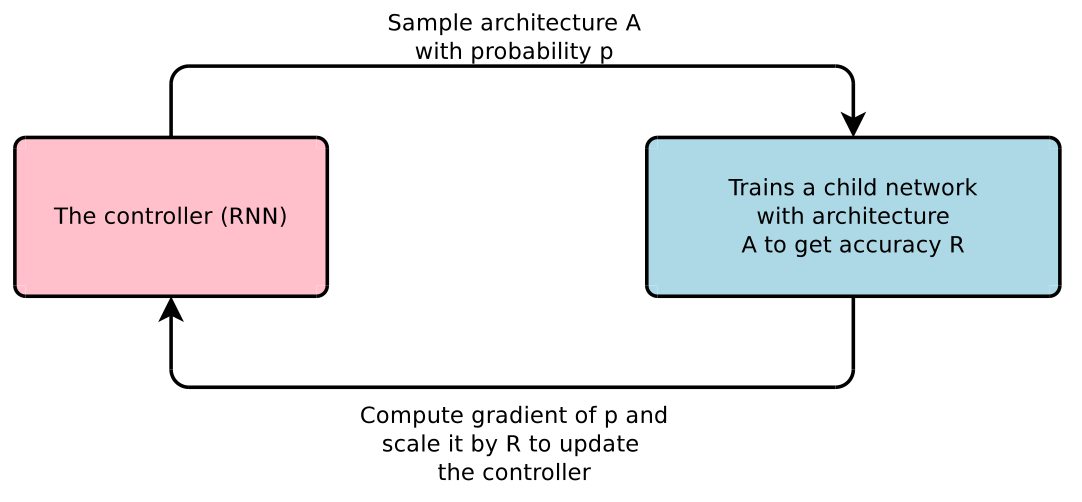
\includegraphics[scale=0.275]{data/zoph-arch-search-overview}
% \end{frame}
% }

% {%
% % A diagram of the action procedure of the RNN controller for creating
% % convnets.
% % Anchor points take skip connections based on sigmoids of tanh's of weighted
% % sums of the previous layer's hidden state and the current (input) layer's
% % hidden state.
% \setbeamertemplate{frame footer}{\cite{neural-architecture-search-45826}}
% \begin{frame}{Neural architecture search: convolutional net}
%         \center{}
%         \vspace{-1.5cm}
%         \hspace*{-1.25cm}
%         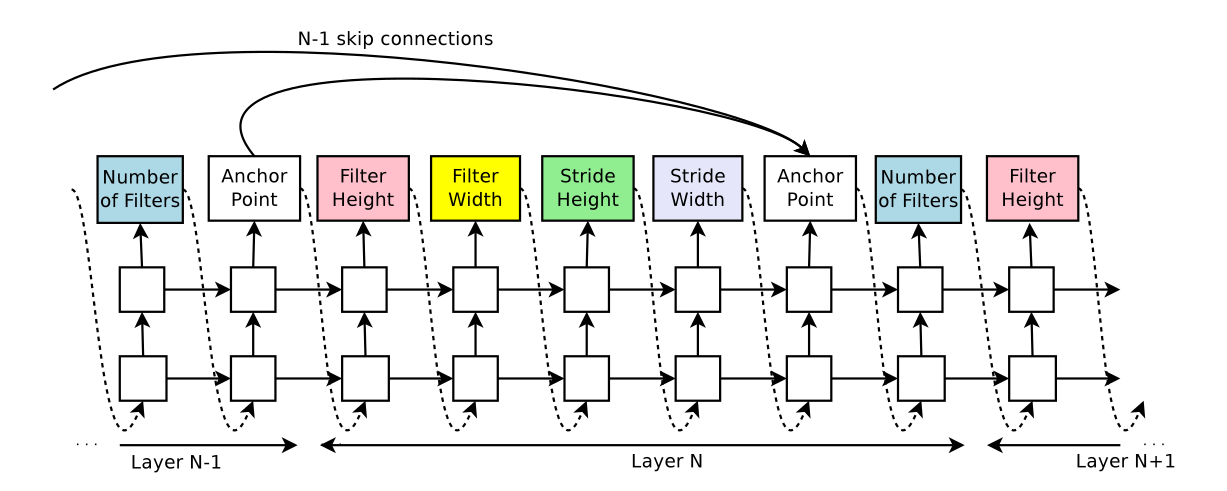
\includegraphics[scale=0.3]{data/neural_arch_convnet}
% \end{frame}
% }

% {%
% % RNNs are generalized into a tree structure.
% % The RNN controller predicts, for each index of the tree, a binary op and
% % unary op (activation), along with tree indices corresponding to the input and
% % output cell states (akin to cell state in LSTMs).
% % This illustration uses base 2, while the true architectures searched over
% % used base 8.
% % Search space for RNNs: 6*10^16. 15000 architectures evaluated.
% \setbeamertemplate{frame footer}{\cite{neural-architecture-search-45826}}
% \begin{frame}{Neural architecture search: RNN}
%         \center{}
%         \vspace{-1.25cm}
%         \hspace*{-1.25cm}
%         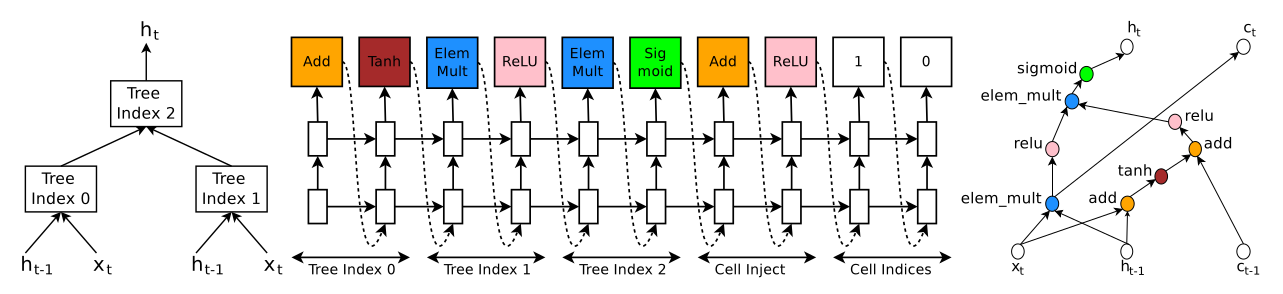
\includegraphics[scale=0.29]{data/neural_arch_rnn}
% \end{frame}
% }

% {%
% \setbeamertemplate{frame footer}{\cite{neural-architecture-search-45826}}
% \begin{frame}{Generated convolutional net}
%         \center{}
%         \vspace{-0.25cm}
%         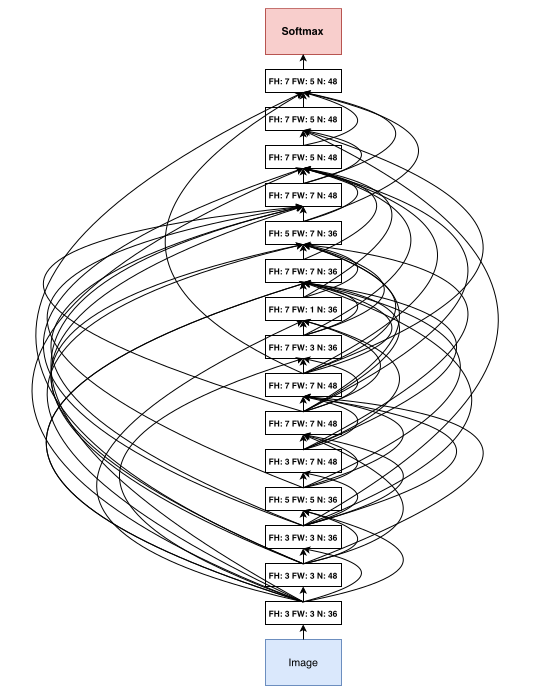
\includegraphics[scale=0.33]{data/neural_arch_convnet_output}
% \end{frame}
% }

% {%
% % The top left is an LSTM. The top right and bottom are generated RNNs,
% % difference being that on the bottom the controller was allowed to use max and
% % sin.
% \setbeamertemplate{frame footer}{\cite{neural-architecture-search-45826}}
% \begin{frame}{Generated RNN}
%         \center{}
%         \vspace{-0.25cm}
%         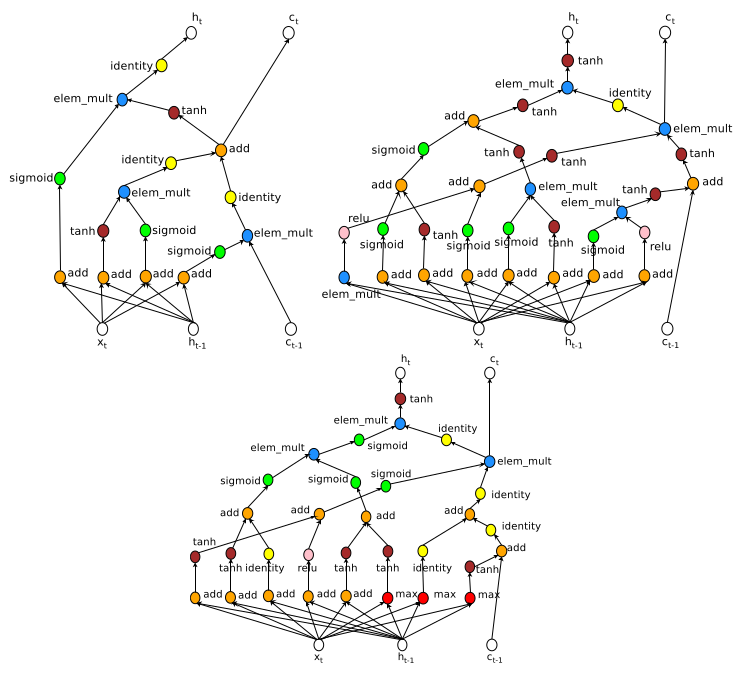
\includegraphics[scale=0.32]{data/neural_arch_rnn_output}
% \end{frame}
% }


\section{Neural Fusion Operator Search}

{%
\begin{frame}{Fusion Op Search Controller}
\centering
\hspace*{-1.0cm}
\scalebox{1.0}{%
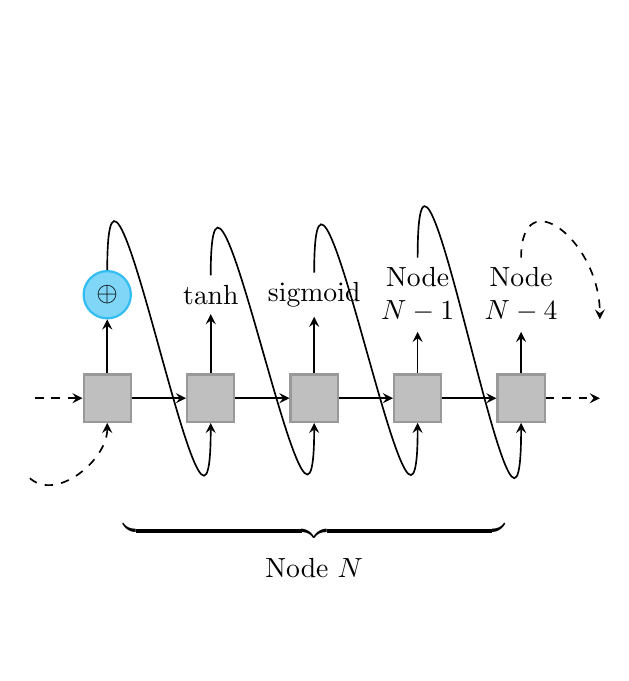
\begin{tikzpicture}
        [oplussty/.style={circle,
                          inner sep=0pt,
                          minimum size=6mm,
                          thick,
                          draw=cyan!80,
                          fill=cyan!50},
         cellsty/.style={rectangle,
                         inner sep=0pt,
                         minimum size=6mm,
                         thick,
                         draw=gray!80,
                         fill=gray!50},
         pre/.style={<-, >=stealth, semithick},
         post/.style={->, >=stealth, semithick}]

        \coordinate (bin op cell coord) at (0mm, 0mm);
        \newcommand{\cellshift}{1cm}

        \node[cellsty] (bin op cell) at (bin op cell coord) {}
                edge [pre, dashed, out=180, in=0] ($(bin op cell coord) + (-1cm, 0mm)$)
                edge [pre, dashed, out=270, in=315] ($(bin op cell coord) + (-1cm, -1cm)$);

        \node[oplussty] (bin op) at (bin op cell.north) [yshift=\cellshift] {$\oplus$}
                edge [pre] (bin op cell);

        \node[cellsty] (func1 cell) at (bin op cell.east) [xshift=\cellshift] {}
                edge [pre] (bin op cell)
                edge [pre, out=270, in=90, looseness=3] (bin op) {};

        \node (func1) at (func1 cell.north) [yshift=\cellshift] {$\tanh$}
                edge [pre] (func1 cell);

        \node[cellsty] (func2 cell) at (func1 cell.east) [xshift=\cellshift] {}
                edge [pre] (func1 cell)
                edge [pre, out=270, in=90, looseness=3] (func1) {};

        \node (func2) at (func2 cell.north) [yshift=\cellshift] {$\sigmoid$}
                edge [pre] (func2 cell);

        \node[cellsty] (node1 cell) at (func2 cell.east) [xshift=\cellshift] {}
                edge [pre] (func2 cell)
                edge [pre, out=270, in=90, looseness=3] (func2) {};

        \node (node1) at (node1 cell.north) [yshift=\cellshift, align=center] {Node\\$N - 1$}
                edge [pre] (node1 cell);

        \node[cellsty] (node2 cell) at (node1 cell.east) [xshift=\cellshift] {}
                edge [pre] (node1 cell)
                edge [pre, out=270, in=90, looseness=3] (node1) {}
                edge [post, dashed, out=0, in=180] ($(node2 cell) + (1cm, 0cm)$);

        \node (node2) at (node2 cell.north) [yshift=\cellshift, align=center] {Node\\$N - 4$}
                edge [pre] (node2 cell)
                edge [post, dashed, out=90, in=90, looseness=2] ($(node2 cell) + (1cm, 1cm)$);

        \node at ($(func2) + (0cm, -3cm)$) {\makebox[32ex]{\upbracefill}};
        \node[inner sep=1pt] at ($(func2) + (0cm, -3cm)$)
                [below, yshift=-3mm] {Node $N$};
\end{tikzpicture}

}
\end{frame}
}

% {%
% \begin{frame}{Tabular Q-learning for fusion operator search}
% \centering
% \hspace*{-12mm}
% 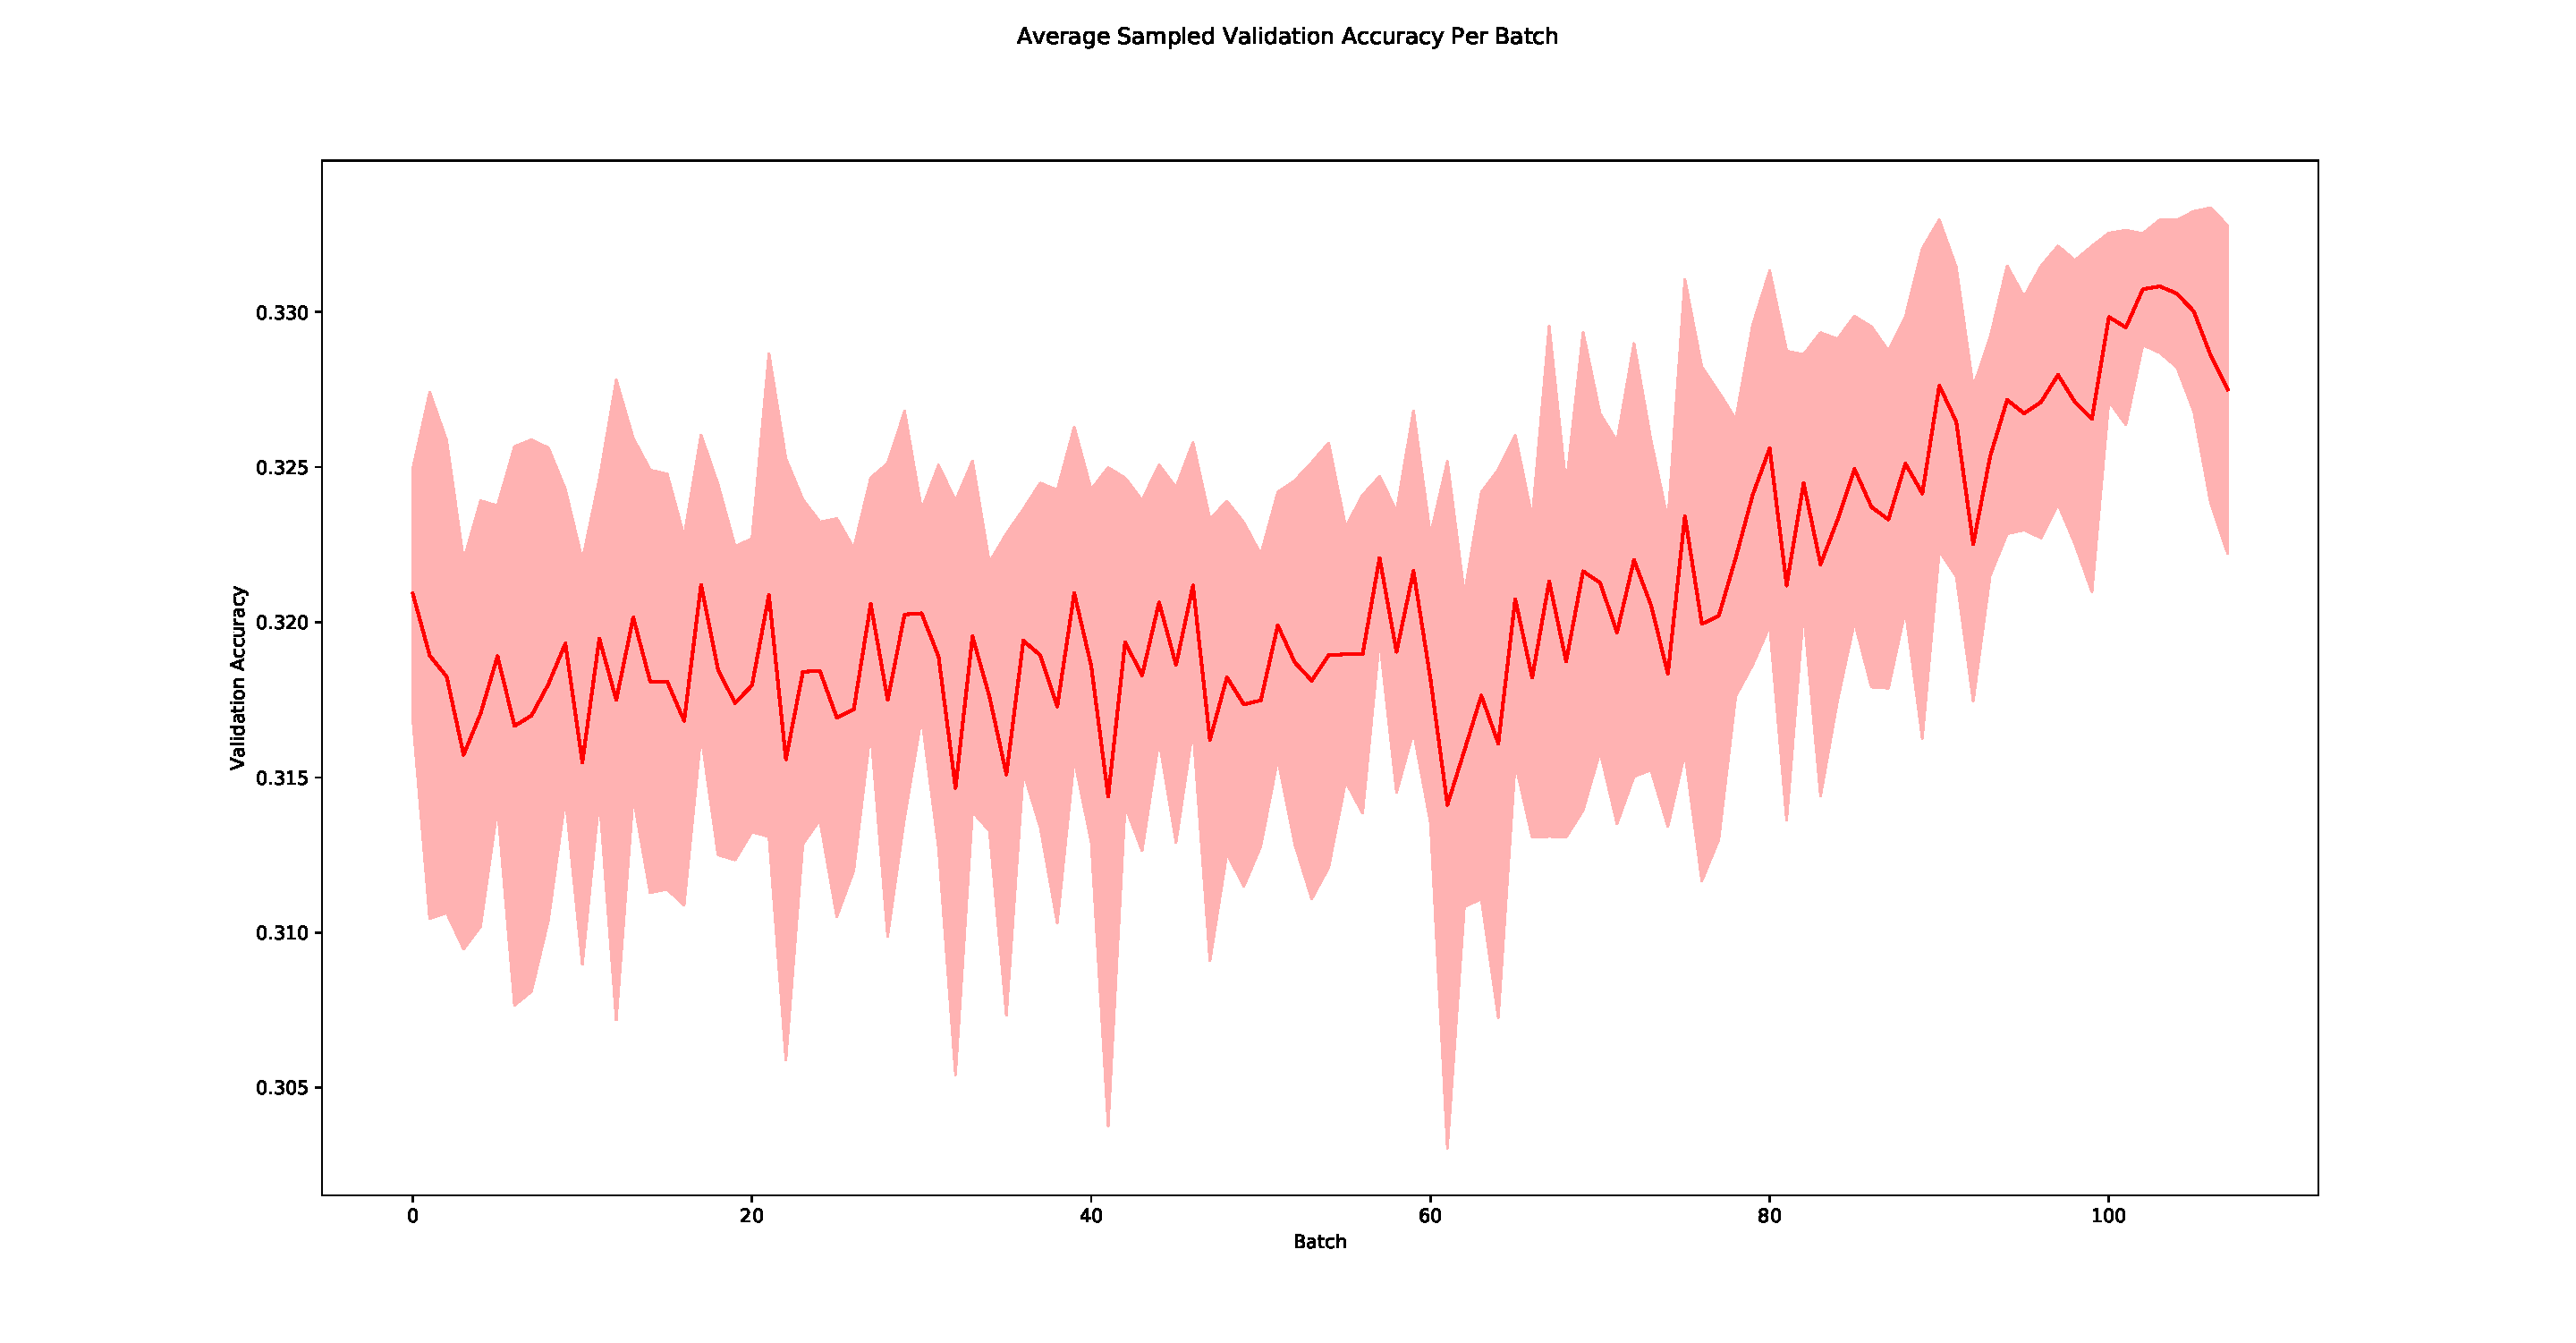
\includegraphics[width=1.2\textwidth]{data/val_accuracy_per_batch.pdf}
% \end{frame}
% }

% \begin{frame}[standout]
%         How about the massive computational cost?
% \end{frame}

% {%
% % Performance follows a log-log scale as dataset size increases (in the linear
% % region)
% % The power law is the same across model architectures, for the same dataset
% \setbeamertemplate{frame footer}{\cite{dlscalingpredictable2017hestness}}
% \begin{frame}{Reduced dataset size for predicting performance}
% \centering
% \hspace*{-6mm}
% 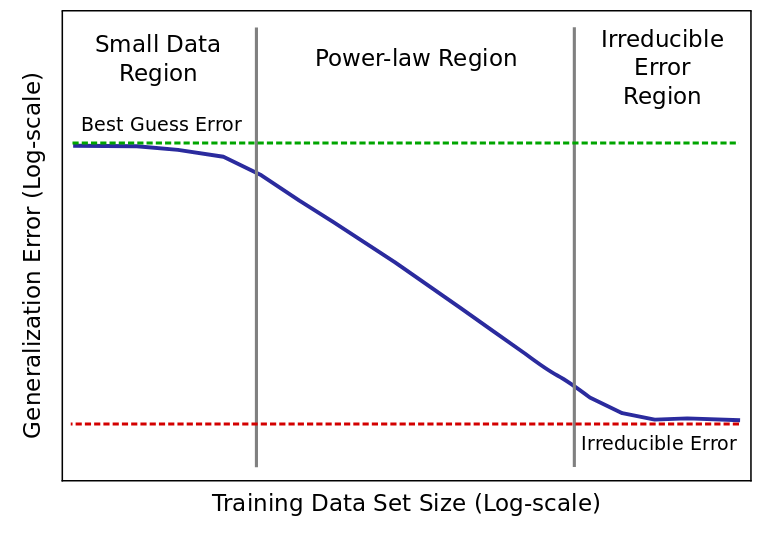
\includegraphics[width=1.1\textwidth]{data/dl-scaling-predictable}
% \end{frame}
% }

% \newcommand{\tildef}{\tilde{f}_i}
% \newcommand{\tildew}{\tilde{w}_i}
% \newcommand{\tildefw}{{\tildef}^{\tildew}}
% \newcommand{\fw}{{f_i}^{w_i}}
% {%
% \setbeamertemplate{frame footer}{\cite{simpleefficient2017elsken}}
% \begin{frame}[fragile]{Network morphisms + RL}
% \centering
% \begin{itemize}[<+- | alert@+>]
% \item (Type I) \\
%         $\tildefw(x) = C(A{f_i}^{w_i}(x) + b) + d$,

% \vspace*{5mm}

% \item (Type II) \\
% $\tildefw(x) = (A \quad\tilde{A}){(h^{w_h}(x) \quad{\tilde{h}}^{w_{\tilde{h}}}(x))}^\intercal + b$,

% \vspace*{5mm}

% \item (Type III) \\
%         $\tildefw(x) = \lambda \fw + (1 - \lambda) h^{w_h}(x)$.
% \end{itemize}
% \end{frame}
% }

\section{Conclusions}

\begin{frame}[fragile]{Conclusions}
        \begin{itemize}[<+- | alert@+>]
                \item Extended strong baseline for fusion in VQA by introducing
                        nonlinear components into the fusion operator.

                \item Policy gradient method for neural fusion operator search.

                % \item Extend to fusion operator search and overcome data
                %         inefficiency:
                %         \begin{itemize}
                %                 \item sample-efficient metalearning methods,

                %                 \item dataset size reduction, and,

                %                 \item ``morphisms''.
                %         \end{itemize}
        \end{itemize}
\end{frame}

\begin{frame}[standout]
        Questions?
\end{frame}

\appendix

\begin{frame}[allowframebreaks]{References}
        \bibliography{fusion-operator}
        \bibliographystyle{apalike}
\end{frame}

\end{document}
